\documentclass[12pt,letterpaper, onecolumn]{exam}
\usepackage{amsmath}
\usepackage{amssymb}
\usepackage[lmargin=71pt, tmargin=1.2in]{geometry}
\usepackage{listings}
\usepackage{color}
\usepackage{graphicx}

\graphicspath{ {./}}

\definecolor{dkgreen}{rgb}{0,0.6,0}
\definecolor{gray}{rgb}{0.5,0.5,0.5}
\definecolor{mauve}{rgb}{0.58,0,0.82}

\lstset{frame=tb,
  language=C,
  aboveskip=3mm,
  belowskip=3mm,
  showstringspaces=false,
  columns=flexible,
  basicstyle={\small\ttfamily},
  numbers=none,
  numberstyle=\tiny\color{gray},
  keywordstyle=\color{blue},
  commentstyle=\color{dkgreen},
  stringstyle=\color{mauve},
  breaklines=true,
  breakatwhitespace=true,
  tabsize=3
}

\lhead{EN.625.252.81 Fall 2025\\}
\rhead{Haadi Majeed\\}
\thispagestyle{empty}

\begin{document}

\begingroup  
    \centering
    \LARGE EN.625.252.81 Fall 2025\\
    \LARGE Module 1 Assignment\\[0.5em]
    \large \today\\[0.5em]
    \large Haadi Majeed\par
    \large hmajeed01\par
    \large Due Sunday August 31st at 10:59 CST\par
\endgroup
\rule{\textwidth}{0.4pt}
\printanswers
\renewcommand{\solutiontitle}{\noindent\textbf{Ans:}\enspace}

\begin{questions}

    \question Find the general solution of the system below two ways:\\
        1) Row reduction by hand.\\
        2) Verify your answer using any program or calculator of your choice. Clearly state which program you used and include a screen shot of your code and output\\
        $$
        \begin{bmatrix}
            1 & 3 & 4 & 7\\
            3 & 9 & 7 & 6
        \end{bmatrix}
        $$
        \begin{solution}
            Multiplying the bottom row by `-3(Row1)'
            $$
            \begin{bmatrix}
                1 & 3 & 4 & 7\\
                3 - 3(1) & 9 - 3(3) & 7 - 3(4) & 6 - 3(7)
            \end{bmatrix}
            $$
            $$
            \begin{bmatrix}
                1 & 3 & 4 & 7\\
                0 & 0 & -5 & -15
            \end{bmatrix}
            $$
            Which can simply to
            $$
            \begin{bmatrix}
                1 & 3 & 4 & 7\\
                0 & 0 & 1 & 3
            \end{bmatrix}
            $$
            This can be turned into Reduced Row Echelon Form by multiplying the top row by `-4(Row2)'
            $$
            \begin{bmatrix}
                1 - 4(0) & 3 - 4(0) & 4 - 4(1) & 7 - 4(3)\\
                0 & 0 & 1 & 3
            \end{bmatrix}
            $$
            Which simplifies to
            $$
            \begin{bmatrix}
                1 & 3 & 0 & -5\\
                0 & 0 & 1 & 3
            \end{bmatrix}
            $$
            $$
            \begin{matrix}
                x_1 + 3x_2 = -5\\
                x_3 = 3
            \end{matrix}
            $$
            $x_2$ is a free variable which results in the following:
            $$
            \begin{matrix}
                x_1 = -5 -3t\\
                x_2 = t\\
                x_3 = 3
            \end{matrix}
            $$\\
            Using the coding language C, I created this program to verify the findings
            \begin{lstlisting}
#include <stdio.h>
#include <stdlib.h>

#define rows 2
#define cols 4

void printMatrix(double matrix[rows][cols])
{
    for (int i = 0; i < rows; i++)
    {
        printf("[ ");
        for (int j = 0; j < cols; j++)
        {
            printf("%7.2f", matrix[i][j]);
        }
        printf(" ]\n");
    }
}

int main() 
{
    double a[rows][cols] = {
        {1.0, 3.0, 4.0, 7.0},
        {3.0, 9.0, 7.0, 6.0}
    };
    printf("Initial state\n");
    printMatrix(a);

    for (int j = 0; j < cols; j++)
    {
        a[1][j] = a[1][j] - 3.0 * a[0][j];
    }
    printf("\nAfter R2 = R2 - 3*R1:\n");
    printMatrix(a);

    double stepConst = -1.0/5.0;
    for (int j = 0; j < cols; j++)
    {
        a[1][j] = stepConst * a[1][j];
    }
    printf("\nAfter R2 = (-1/5)*R2:\n");
    printMatrix(a);

    for (int j = 0; j < cols; j++)
    {
        a[0][j] = a[0][j] - 4.0 * a[1][j];
    }
    printf("\nAfter R1 = R1 - 4*R2 (Reduced Row Echelon Form):\n");
    printMatrix(a);

}
        \end{lstlisting}
        And this is the output when compiled and executed\\
        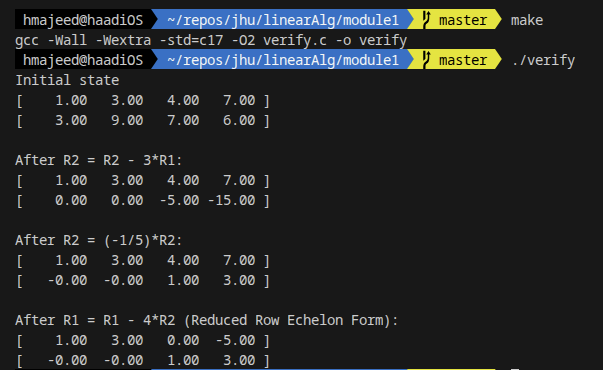
\includegraphics{code-tested}
        \end{solution}
    % end question 1

    \question What would you have to know about the pivot columns in an augmented
        matrix in order to know that the linear system is consistent and has a
        unique solution? Explain in complete sentences and provide examples to
        justify your reasoning.
    
        \begin{solution}
            For a linear system to be consistent, the last column pf the augmented matrix must not be a pivot. In addition to that, if it is unique, that means every column (variable) has a single pivot. The following is an example of such.

            $$
            \begin{bmatrix}
                1 & 0 & 3\\
                0 & 1 & 7
            \end{bmatrix}
            $$

            An example that would not be consistent nor have pivots for every column would be as follows.
            
            $$
            \begin{bmatrix}
                1 & 0 & 3 & 5\\
                0 & 1 & 7 & 2\\
                0 & 0 & 0 & 3
            \end{bmatrix}
            $$
        \end{solution}
    % end question 2

    \question Consider the linear system\\
            $$
            \begin{matrix}
                x_1 + hx_2 = 2\\
                4x_1 + 8x_2 = k
            \end{matrix}
            $$
            \begin{parts}
            \part Find values of \emph{h} and \emph{k} such that the system has no solution
            \part Find values of \emph{h} and \emph{k} such that the system has a unique solution.
            \part Find values of \emph{h} and \emph{k} such that the system has infinitely many solutions.
        \end{parts}
        \begin{solution}
            $$
            \begin{bmatrix}
                1 & h & 2\\
                4 & 8 & k
            \end{bmatrix}
            $$
            $R_2 \leftarrow R_2 - 4(R_1)$
            $$
            \begin{bmatrix}
                1 & h & 2\\
                4 - 4(1) & 8 - 4(h) & k - 4(2)
            \end{bmatrix}
            $$
            $$
            \begin{bmatrix}
                1 & h & 2\\
                0 & 8 - 4h & k - 8
            \end{bmatrix}
            $$
            \begin{parts}
                \part 
                    $(8-4h)x_2 = k - 8$\\
                    So $8 - 4h = 0$ and $k - 8 \neq 0$\\
                    For no solution, $h = 2$ and $k = 8$
                \part 
                    As long as the coefficient of $x_2$ is nonzero $k - 8$ can be any value, therefore:\\
                    $h \neq 2$ and $k$ can be any real number
                \part
                    To have infinite solutions, it must be consistent and one free variable.\\
                    Using 
                    $
                    h = 2 \rightarrow 
                    \begin{bmatrix}
                        1 & 2 & 2\\
                        0 & 0 & k - 8     
                    \end{bmatrix}
                    $
                    to be consistent, $ k - 8$ must also equal 0, thus $ k = 8 \rightarrow
                    \begin{bmatrix}
                        1 & 2 & 2\\
                        0 & 0 & 0
                    \end{bmatrix}
                    $\\
                    Resulting in $x_1 + 2x_2 = 2 \rightarrow x_1 = 2 - 2x_2$ with infinite solutions for $h = 2$ and $k = 8$

            \end{parts}
        \end{solution}
    % end question 3
    
\end{questions}
\end{document}